% IMPORTANT: PLEASE USE XeLaTeX FOR TYPESETTING
\documentclass{sintefbeamer}
\usepackage{xeCJK}

\makeatletter
\setbeamertemplate{footline}
{
  \leavevmode%
  \hbox{%
  \begin{beamercolorbox}[wd=.5\paperwidth,ht=2.25ex,dp=1ex,center]{title in head/foot}%
    \usebeamerfont{title in head/foot}基于联邦学习的轨迹大数据隐私保护方案研究
  \end{beamercolorbox}%
  \begin{beamercolorbox}[wd=.5\paperwidth,ht=2.25ex,dp=1ex,right]{date in head/foot}%
    \usebeamerfont{date in head/foot}\insertshortdate{}\hspace*{2em}
    \insertframenumber{} / \inserttotalframenumber\hspace*{2ex} 
  \end{beamercolorbox}}%
  \vskip0pt%
}
\makeatother

% meta-data
\title{基于联邦学习的轨迹大数据隐私保护方案研究 }
\subtitle{答辩人:黄其涵 \qquad 导师:章静 教授\qquad 学科专业:电子信息 }
%\author{黄其涵}
\date{2022 年 12 月 25 日}
\titlebackground{images/bg4}

% document body
\begin{document}

\maketitle

\section{选题依据}{}

\begin{frame}{1.1 选题背景及意义}{\thesection \, \secname}
\begin{columns}
\begin{column}{0.4\textwidth}
\begin{figure}[ht]
\centering
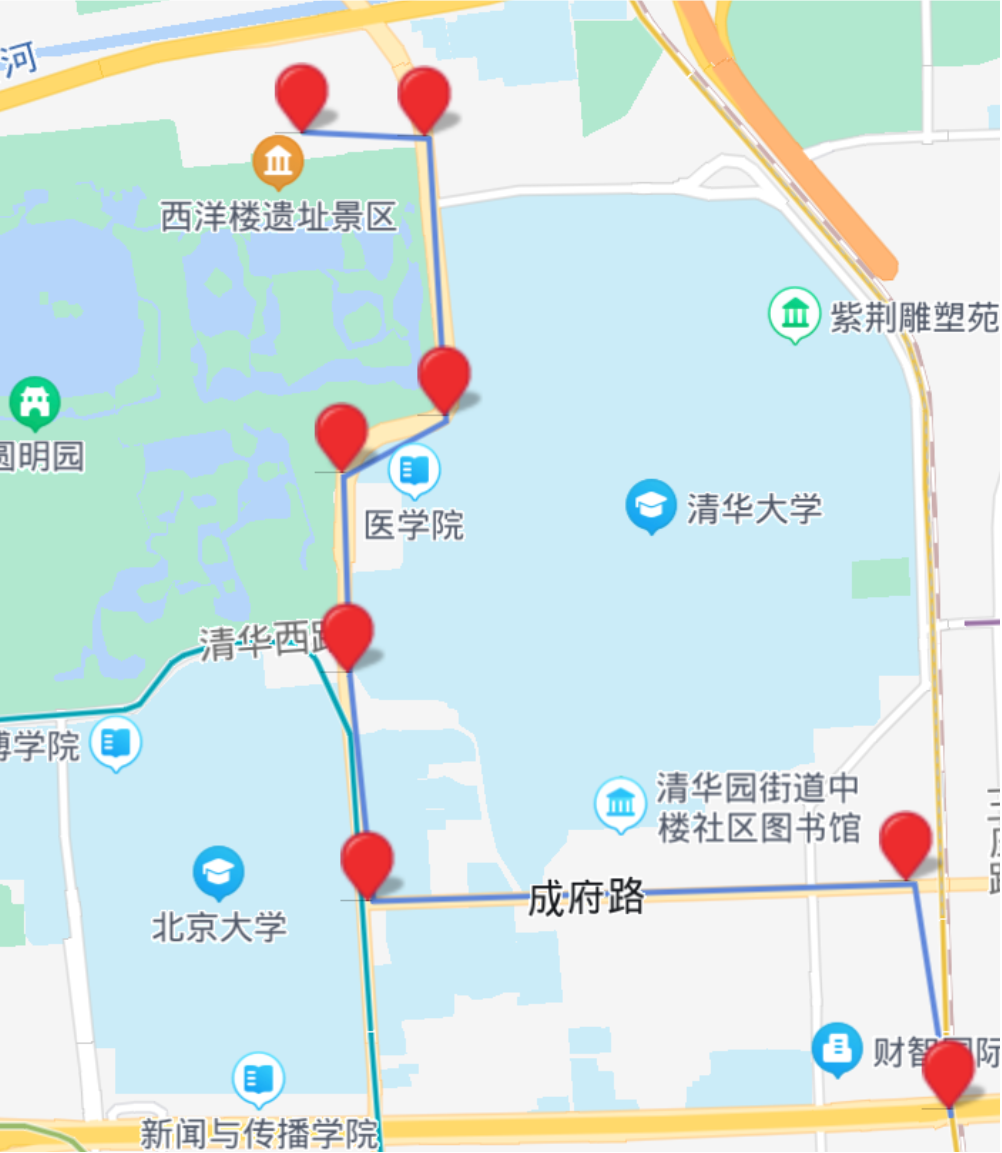
\includegraphics[width=0.8\textwidth]{images/real_traj}
\end{figure}
\end{column}
\begin{column}{0.6\textwidth}
\textbf{基于位置的服务(LBS)会产生大量的轨迹数据}
\begin{itemize}
	\item 轨迹数据包含了人们的出行方式及其与城市环境相互作用的丰富信息,可被用于研究交通堵塞分析、出行模式与行为分析、位置兴趣点个性化推荐等;
	\item 然而,轨迹可能会较为准确地揭示用户的行为模式,从而允许攻击者推断用户较为敏感的生活隐私,其中包括健康状况、社会关系与宗教信仰等;
	\item \textbf{\alert{保护轨迹隐私的同时又保留数据可用性}},这已然成为当今世界亟待解决的社会问题。
\end{itemize}
\end{column}
\end{columns}
\end{frame}

\begin{frame}{1.2 国内外研究现状}
传统的轨迹数据隐私保护方案主要基于泛化的$k$匿名方法以及基于扰动的差分隐私方法。近年来,基于机器学习的一些轨迹隐私保护方案逐渐兴起,他们通常用来高效地处理大规模的轨迹数据以降低人工成本。
\begin{itemize}
\item \textbf{基于泛化方法的隐私保护方案}
  \begin{itemize}
  \item 优点:容易实现,能够抵御一定程度的链接攻击。
  \item 缺点:高度依赖背景知识与专家能力,隐私性与效用性之间的权衡难以控制。
  \end{itemize}
\item \textbf{基于扰动方法的隐私保护方案}
  \begin{itemize}
  \item 优点:可量化的隐私保护方法,能有效地减少基于背景知识攻击的影响。
  \item 缺点:对模型可用性影响较大,隐私预算设定不易度量。
  \end{itemize}
\end{itemize}
\textbf{基于联邦学习的隐私保护方法}允许在多个参与者之间共享训练数据而不会泄露其数据隐私,是能够解决“数据孤岛”问题的隐私保护技术,是新时代新问题的解决方案。
\end{frame}

\section{研究内容}

\begin{frame}{研究内容框架}

\begin{columns}
\begin{column}{0.5\textwidth}
\vspace*{-0.4cm} \begin{block}{\textbf{1 社会问题}}\centering
\textbf{保护轨迹隐私的同时保留数据可用性}
\end{block}
\end{column}
\begin{column}{0.5\textwidth}
\vspace*{-0.4cm} \begin{block}{\textbf{2 科学问题}}\centering
\textbf{不同场景下的轨迹隐私保护技术研究}
\end{block}
\end{column}
\end{columns}

\vspace*{0.2cm} \hspace*{-0.7cm} 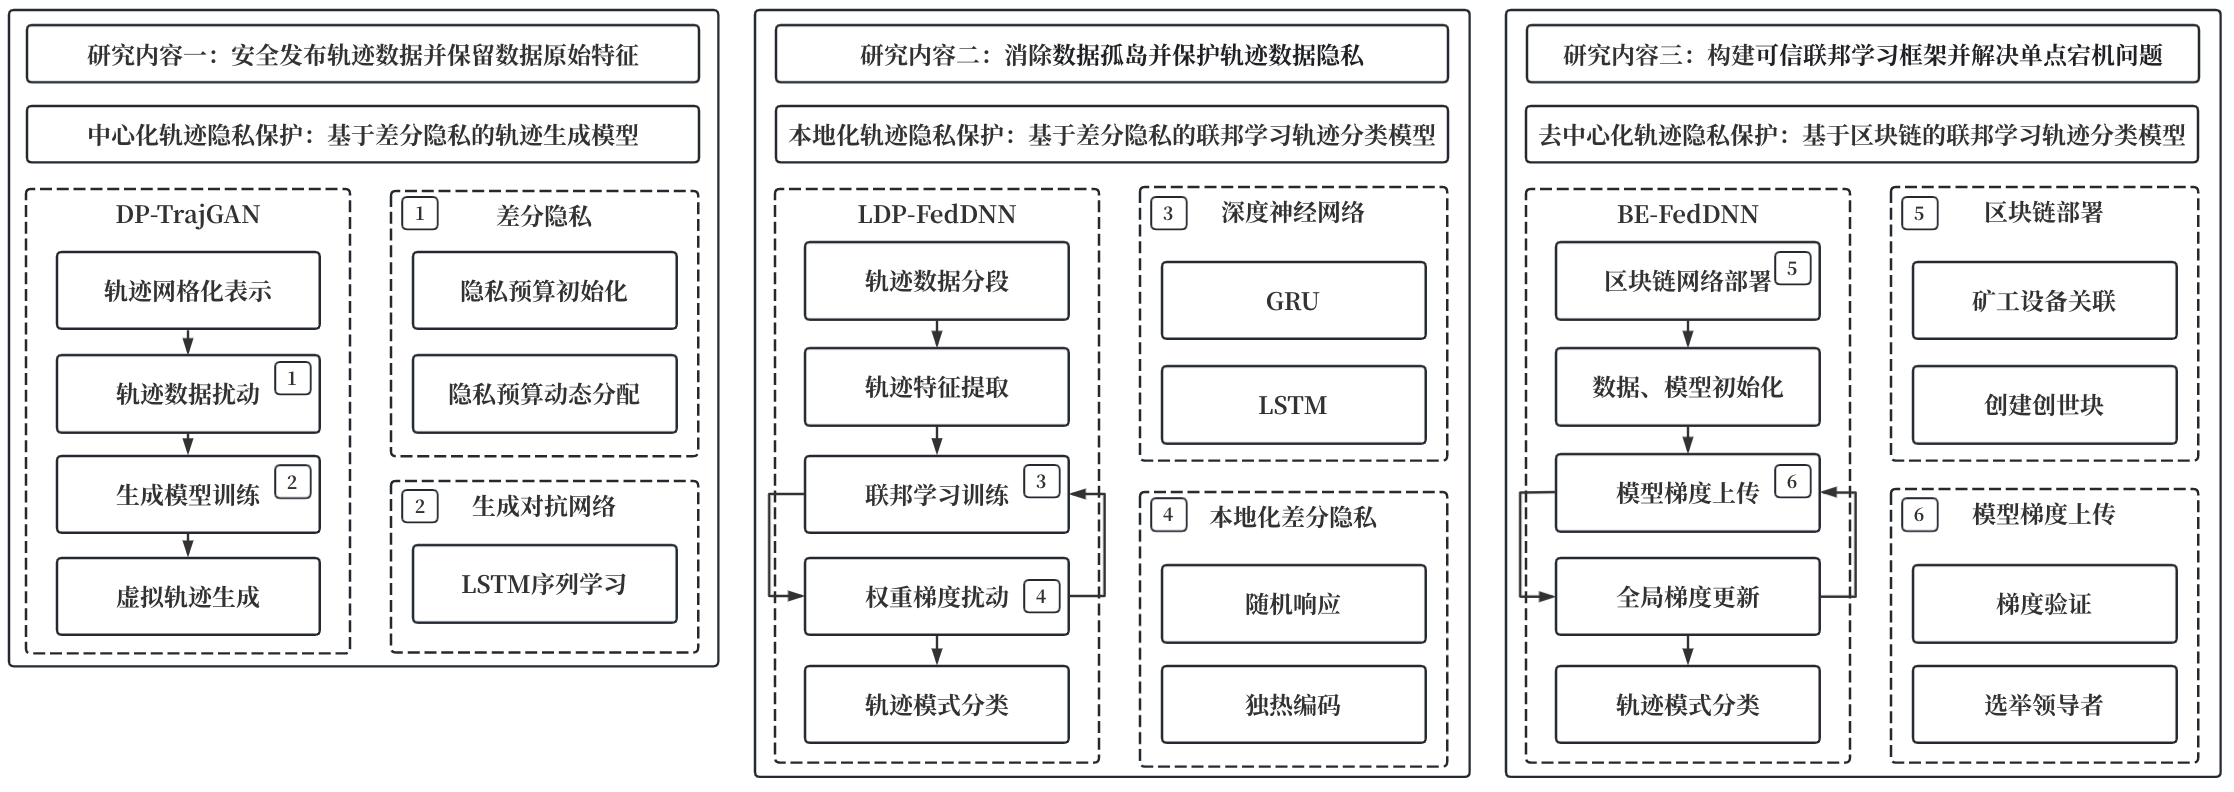
\includegraphics[width=1.1\textwidth]{images/content}
\end{frame}

\section{研究方案}

\begin{frame}{3.1 基于差分隐私的轨迹生成模型}
\begin{columns}
\begin{column}{0.5\textwidth}
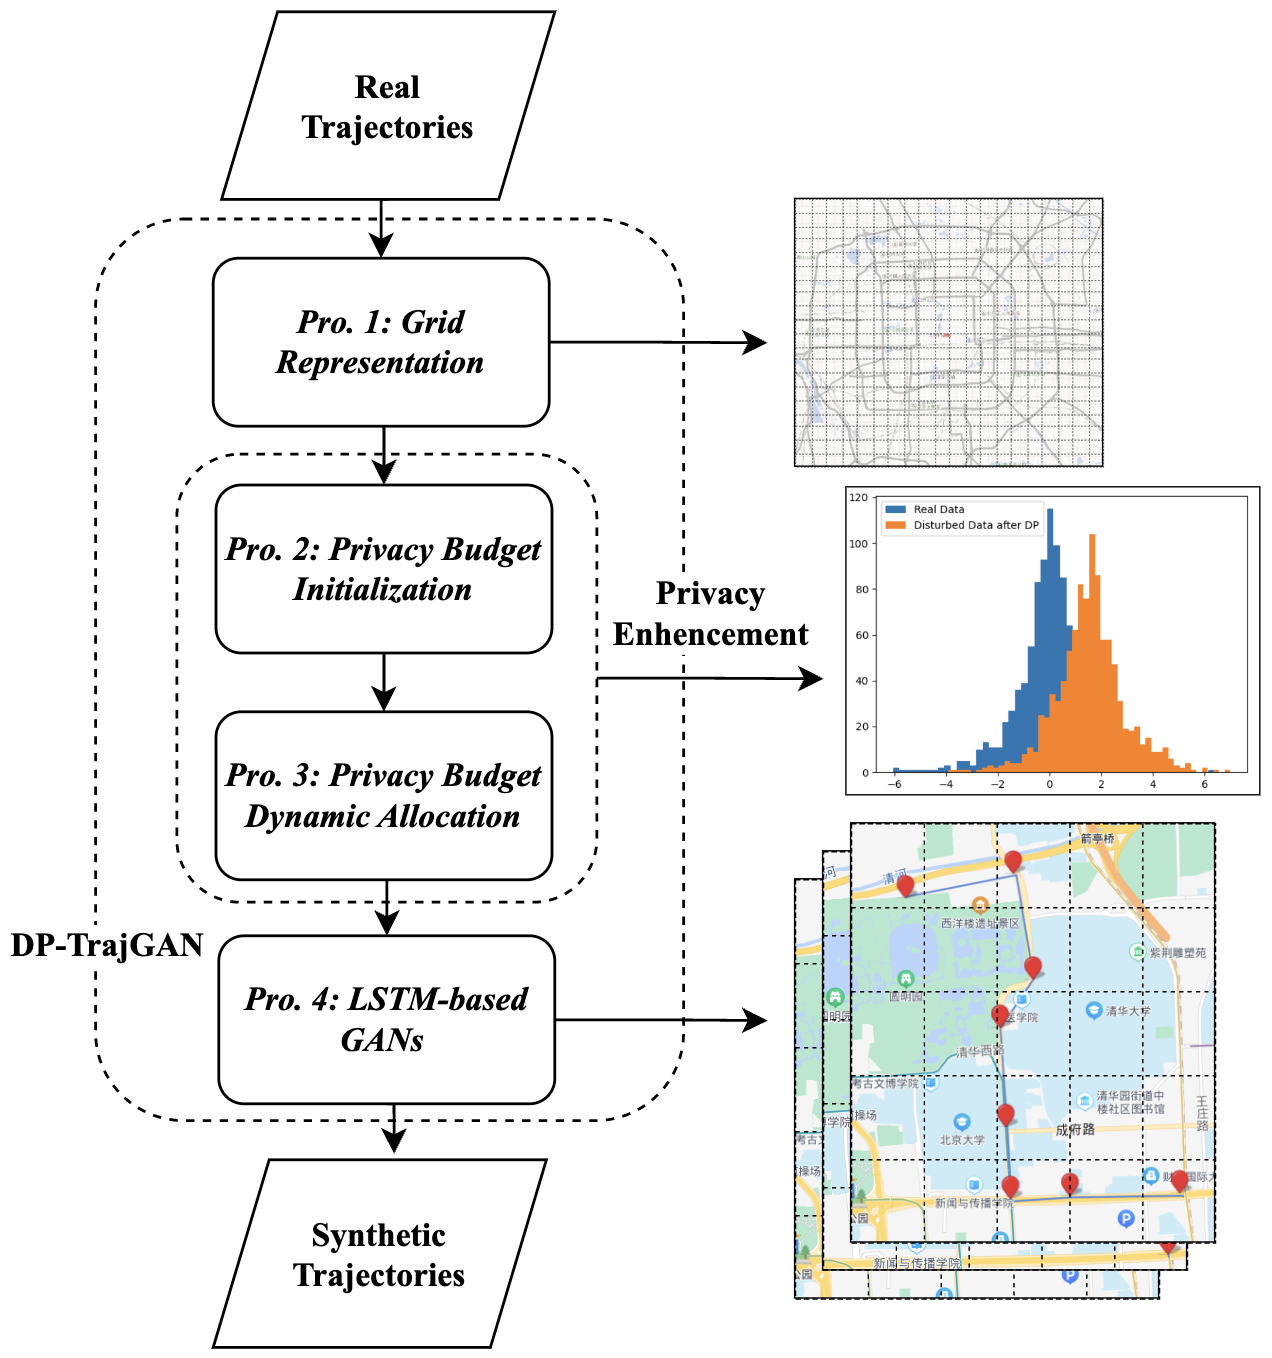
\includegraphics[height=1\textheight]{images/survey1}
\end{column}
\begin{column}{0.5\textwidth}
\begin{itemize}
  \item[Step 1] 轨迹网格化表示
$\text { traj }=\left\{r_{t 1}, r_{t 2}, \ldots, r_{t j}\right\}, \forall r_{t j} \in R$
  \item[Step 2] 时空隐私预算初始化\\
  (1)基于轨迹空间密度扰动位置坐标\\
空间总隐私预算分配:\\$\varepsilon_s=\sum_{i=1}^{c_r^{l a t} * c_r^{\operatorname{lng}}} \varepsilon_s^i$\\
每网格的空间隐私预算分配:\\$\varepsilon_S^i=\frac{e^{\operatorname{den}\left(r_i\right)}}{\sum_{i=1}^{c_r^{l a t} *_r \operatorname{lng}} e^{\operatorname{den}\left(r_j\right)}}$\\
 (2)基于轨迹时间密度扰动位置时刻\\
时间总隐私预算分配:\\$\varepsilon_t=\sum_{i=1}^{c_r^{l a t} * c_r^{\operatorname{lng}}} \sum_{j=1}^{48} \varepsilon_t^{i j}$\\
每网格的时间隐私预算分配:\\
  $\varepsilon_t^{i j}=\frac{e^{f r e q^{-1}\left(r_i, \text { range }_j\right)}}{\sum_{a=1}^{c_r^{l a t} * c_r^{\operatorname{lng}}} \sum_{b=1}^{48} e^{f r e q^{-1}\left(r_a, \text { range }_b\right)}}$

 \end{itemize}
\end{column}
\end{columns}
\end{frame}

\begin{frame}{3.1 基于差分隐私的轨迹生成模型}
\begin{columns}
\begin{column}{0.5\textwidth}
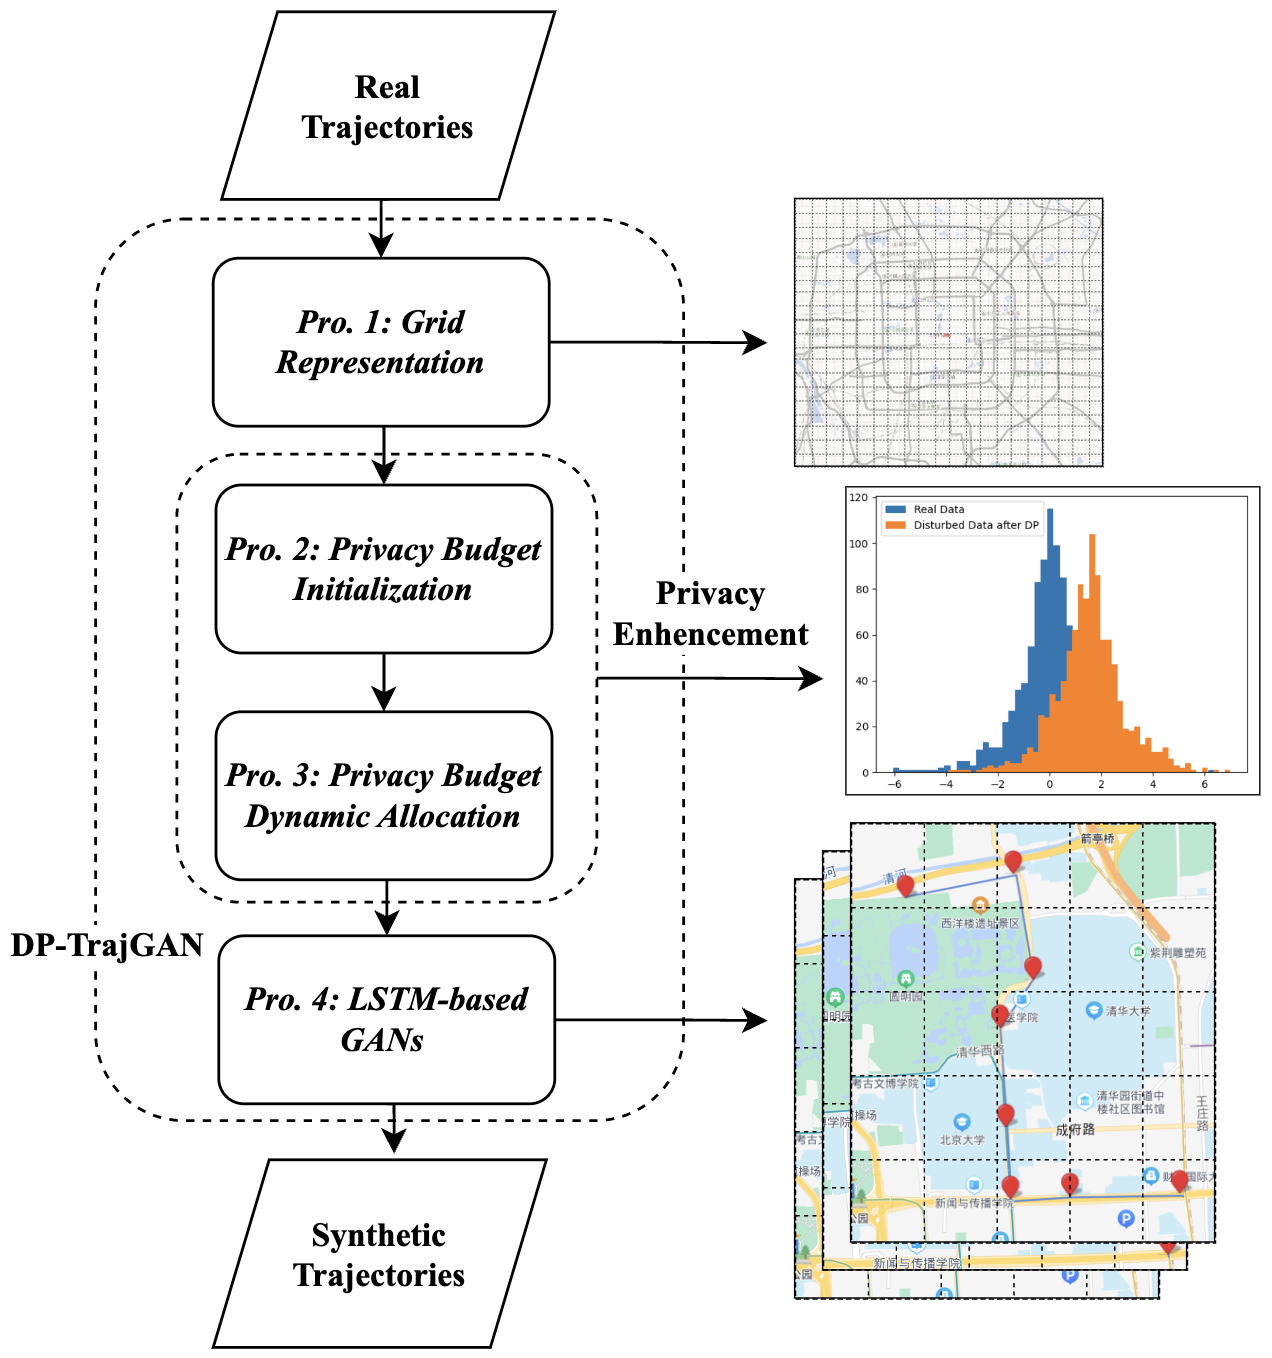
\includegraphics[height=1\textheight]{images/survey1}
\end{column}
\begin{column}{0.5\textwidth}
\begin{itemize}
  \item[Step 1] 轨迹网格化表示
  \item[Step 2] 时空隐私预算初始化
  \item[Step 3] 时空隐私预算动态分配
  	\begin{itemize}
  	\item 基于POMDP进行隐私预算\\自适应分配:
  	$\max E\left[\sum_{t=0}^{\infty} \gamma^t \mathcal{R}\left(s_t, a_t\right)\right]$\\
  	其中 $\gamma \in [0,1]$是折扣系数,$\mathcal{R}$ 是奖励函数,$s$ 是可观察状态,$a$ 是执行的行动。
  	\end{itemize}
  	
  \item[Step 4] 轨迹生成对抗网络训练
  	\begin{itemize}\item 使用LSTM-based GANs进行 \\轨迹序列学习 \end{itemize}
 \end{itemize}
\end{column}
\end{columns}
\end{frame}

\begin{frame}{3.1.1 LSTM-based GANs 架构}
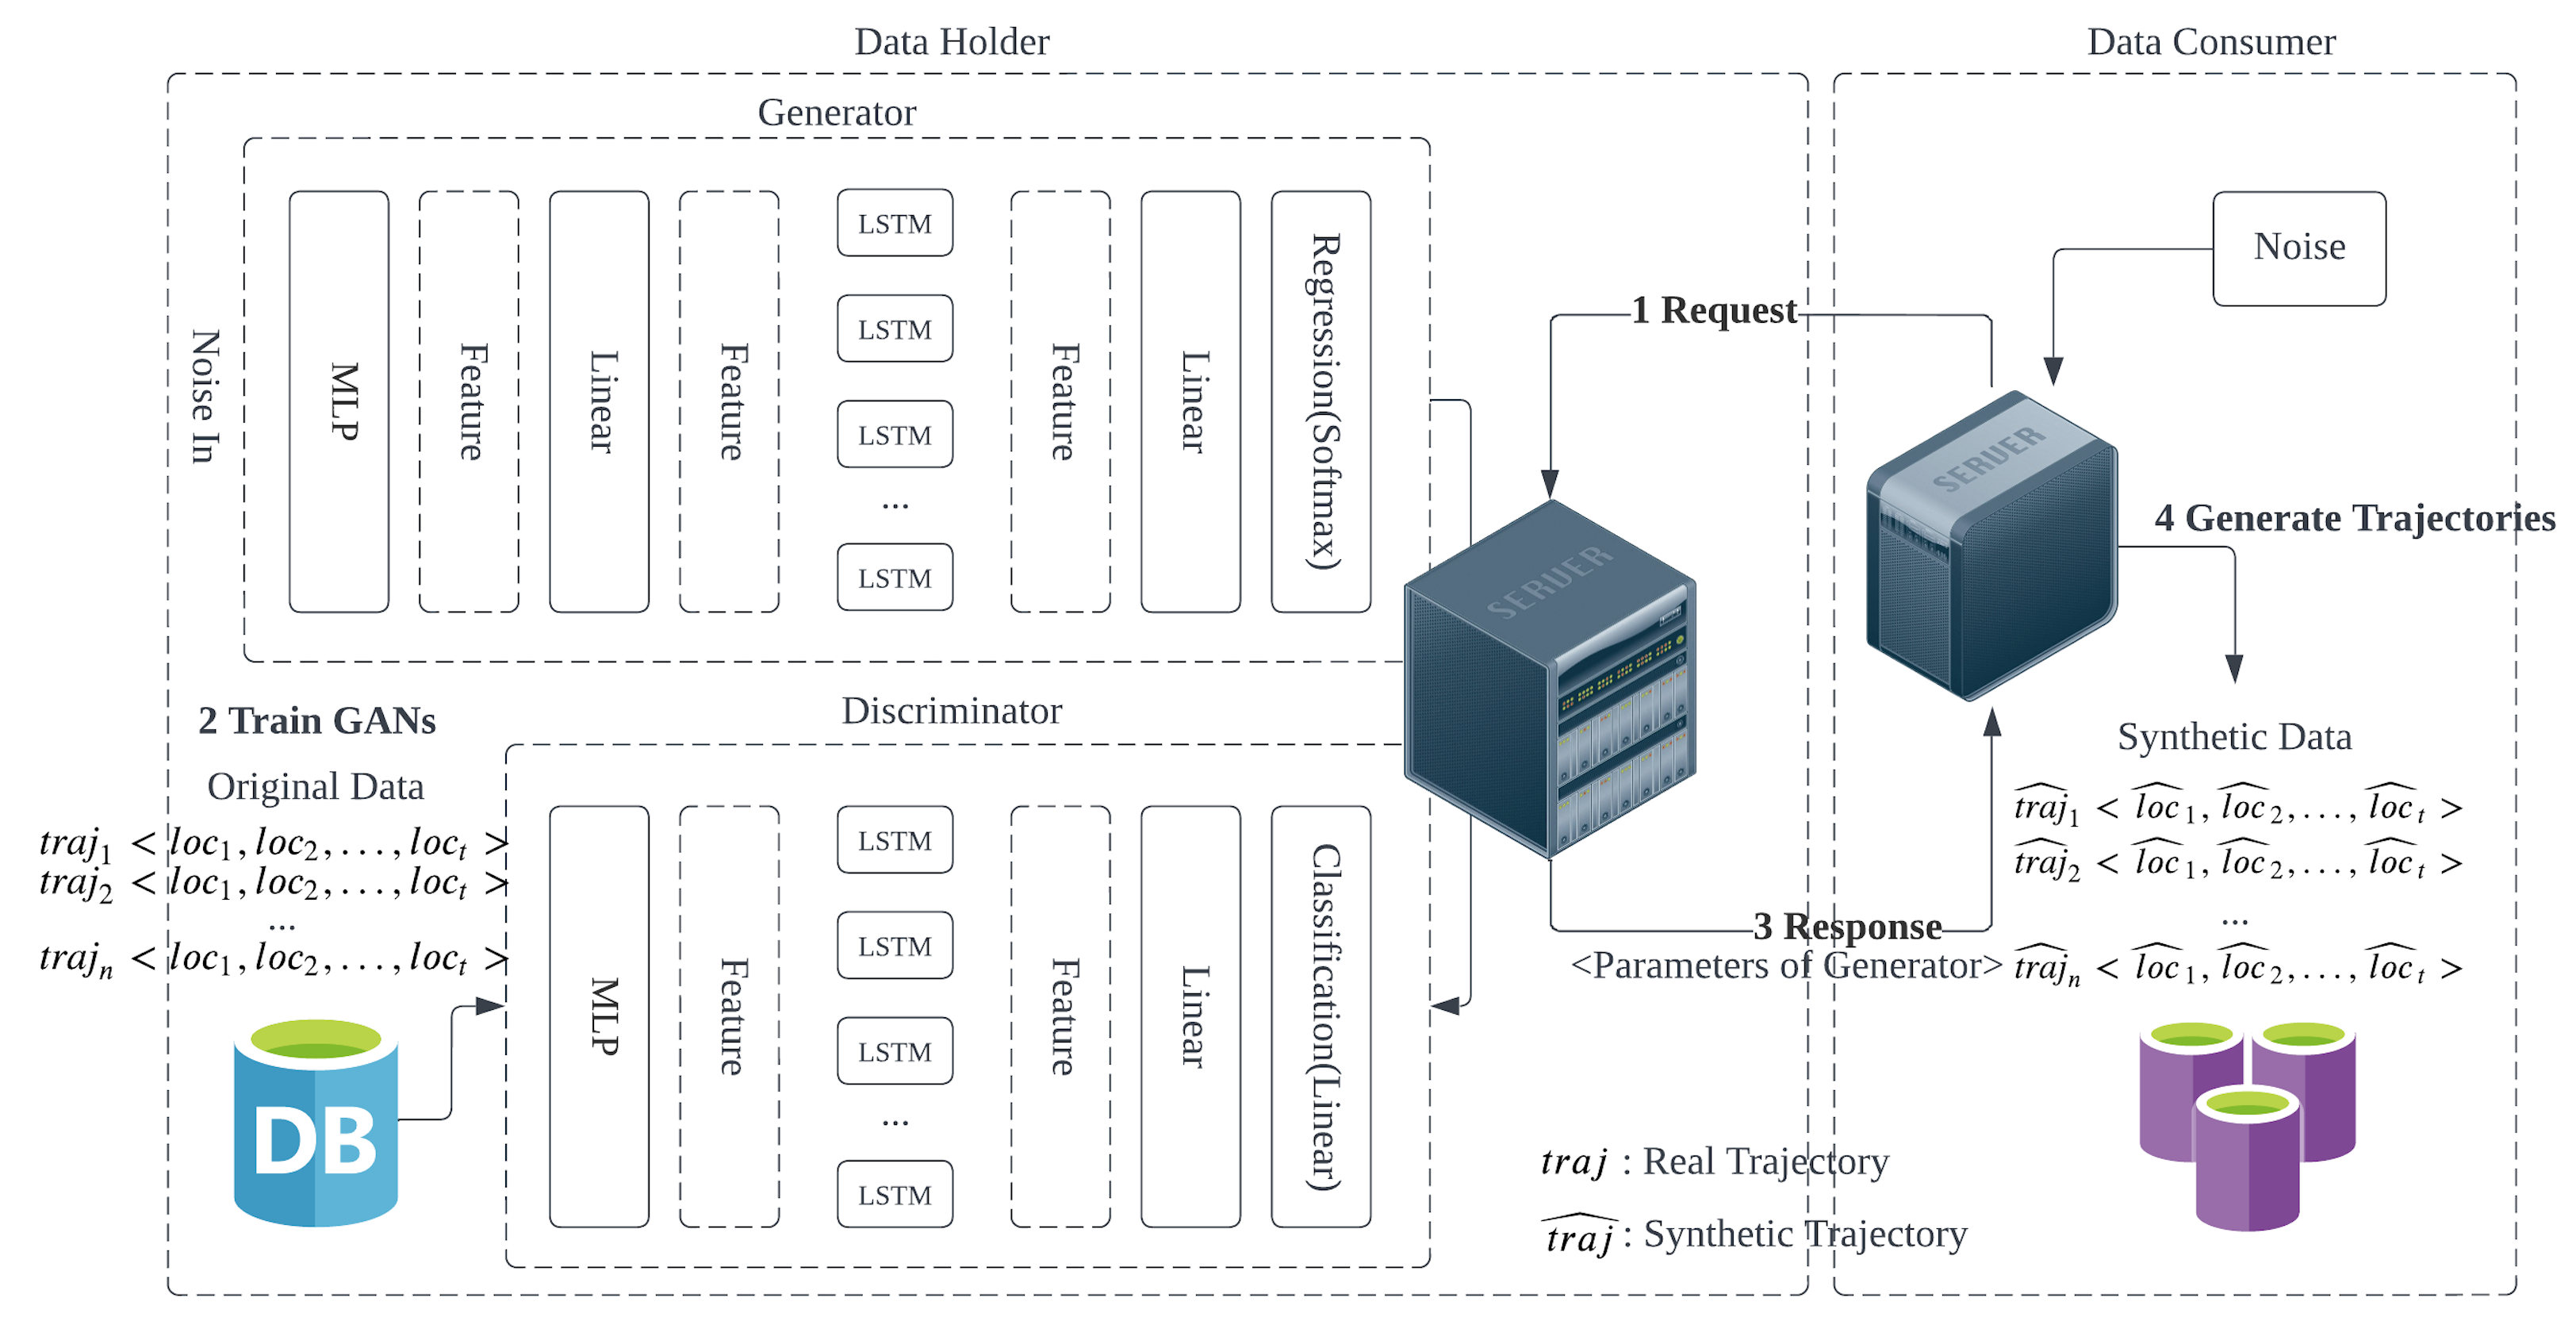
\includegraphics[width=0.95\textwidth]{images/survey1-1}
\end{frame}


\begin{frame}{3.2 基于差分隐私的联邦学习轨迹分类模型}
\begin{columns}
\begin{column}{0.55\textwidth}
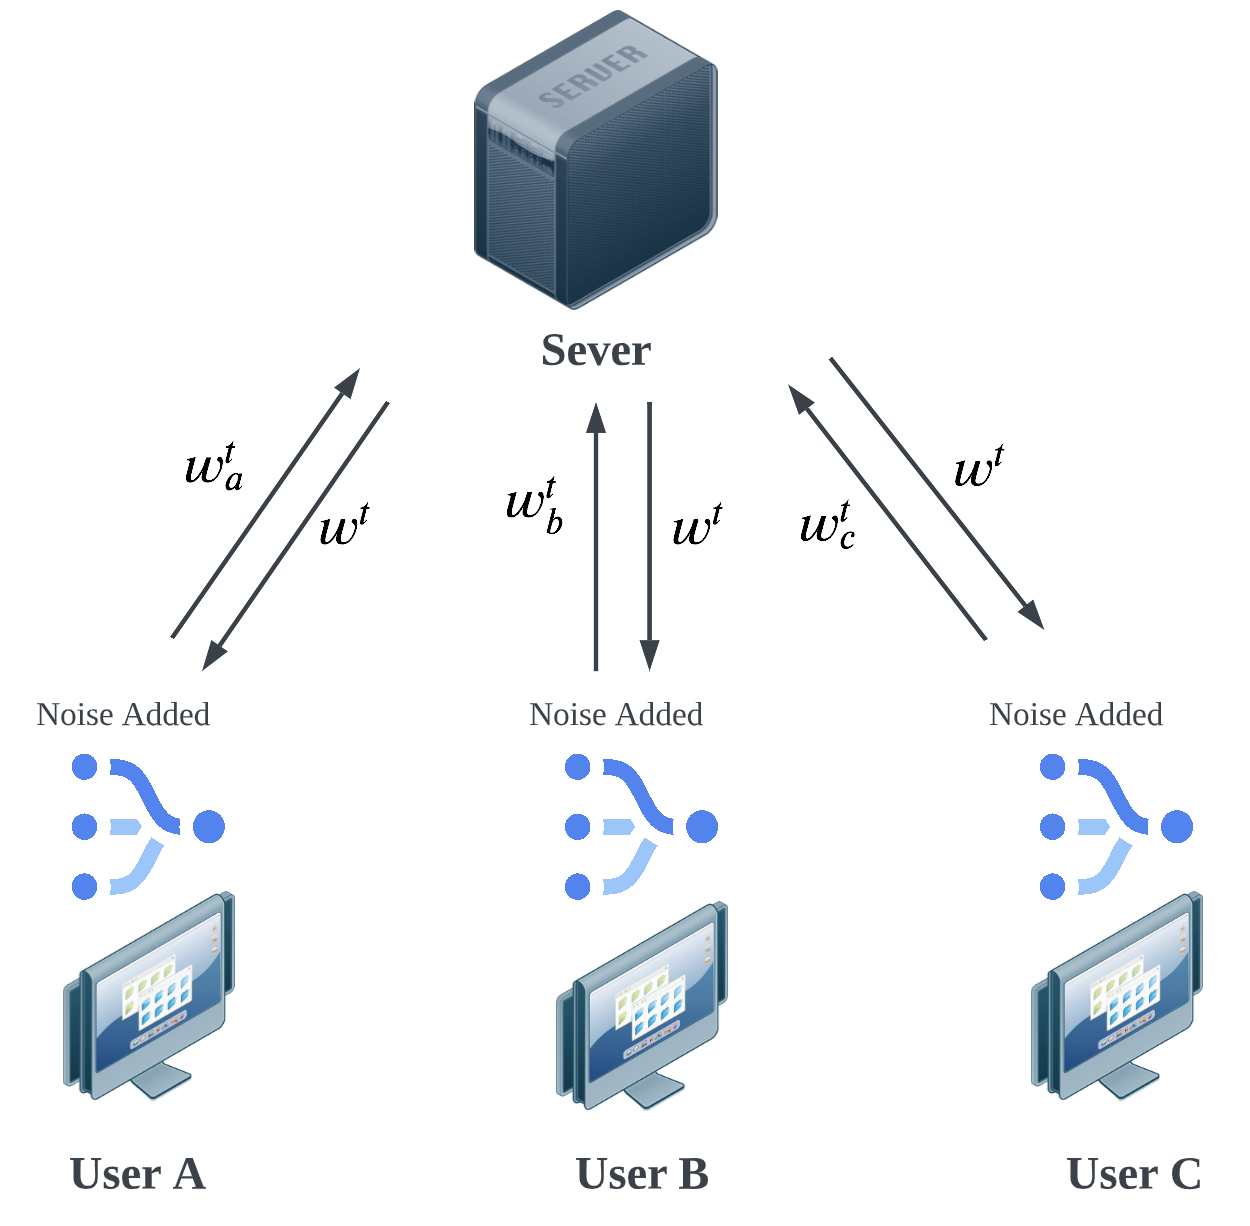
\includegraphics[height=1\textheight]{images/fl}
\end{column}
\begin{column}{0.45\textwidth}
\begin{itemize}
  \item[Tech 1] 联邦学习(FL)
  \begin{itemize}
   \item 数据不动,模型动
   \item 解决“数据孤岛”问题
   \item 提高模型鲁棒性
  \end{itemize}
  \item[Tech 2] 本地化差分隐私(LDP)
  \begin{itemize}
  \item 权重梯度扰动
  \item 避免攻击者通过梯度反推样本
  \item 防止模型过拟合
  \end{itemize}
 \end{itemize}
\end{column}
\end{columns}
\end{frame}

\begin{frame}{3.2.1 轨迹分类任务}
\begin{columns}
\begin{column}{0.4\textwidth}\centering
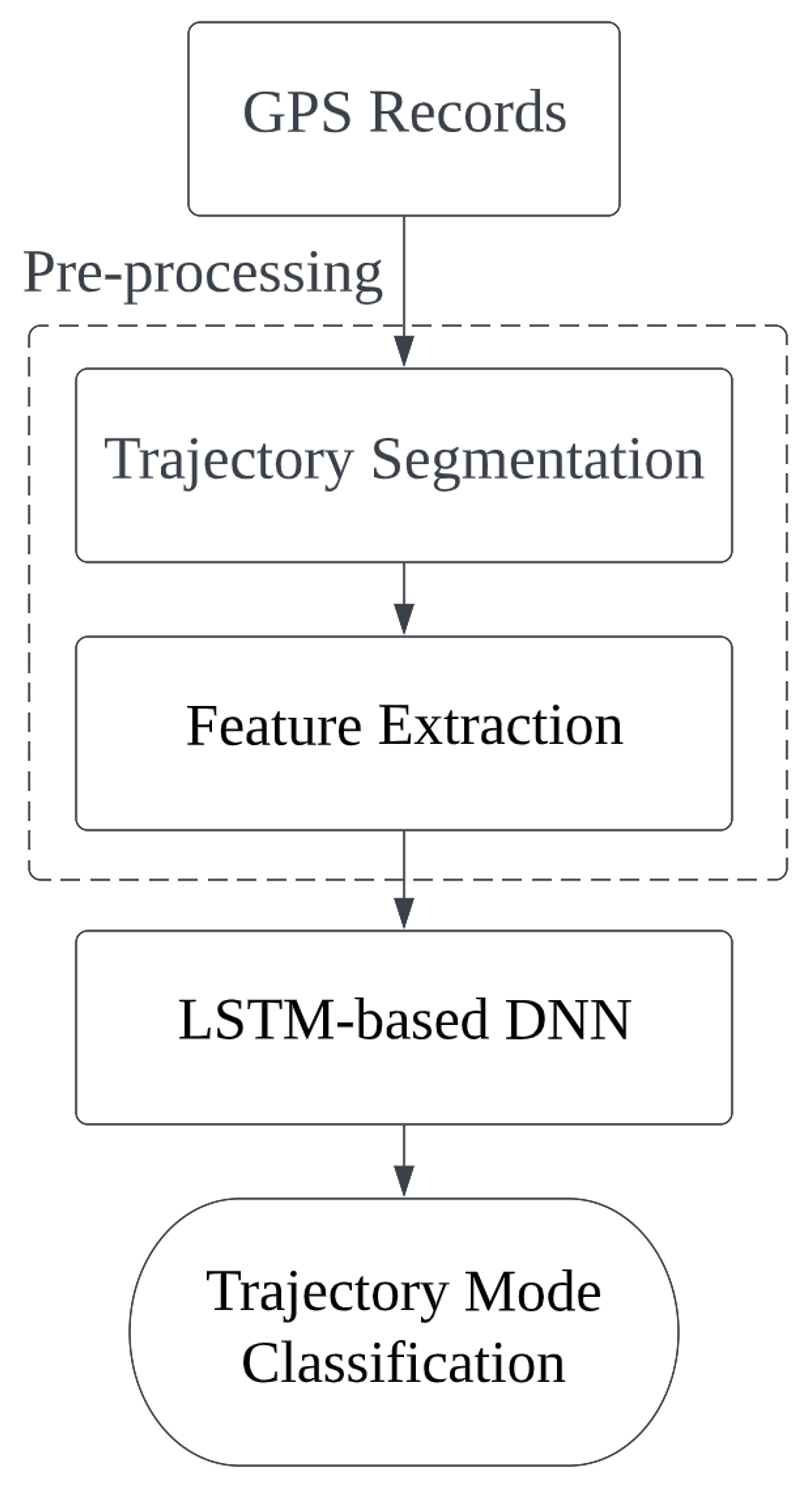
\includegraphics[height=1\textheight]{images/traj-cls}
\end{column}
\begin{column}{0.6\textwidth}
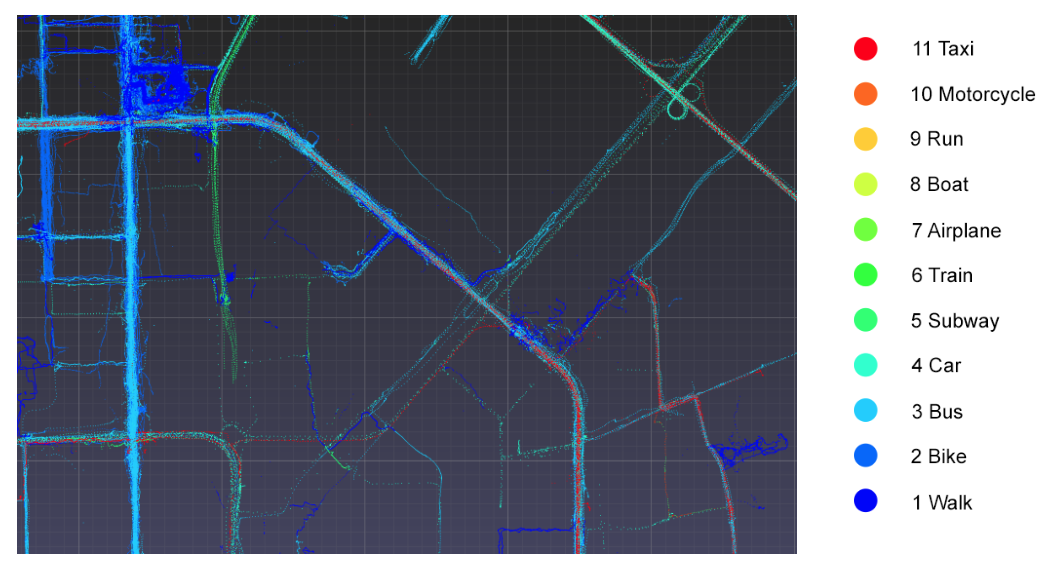
\includegraphics[width=1\textwidth]{images/tul-cls}
\end{column}
\end{columns}
\end{frame}

\begin{frame}{3.3 基于区块链的联邦学习轨迹分类模型}
\begin{columns}
\begin{column}{0.6\textwidth}
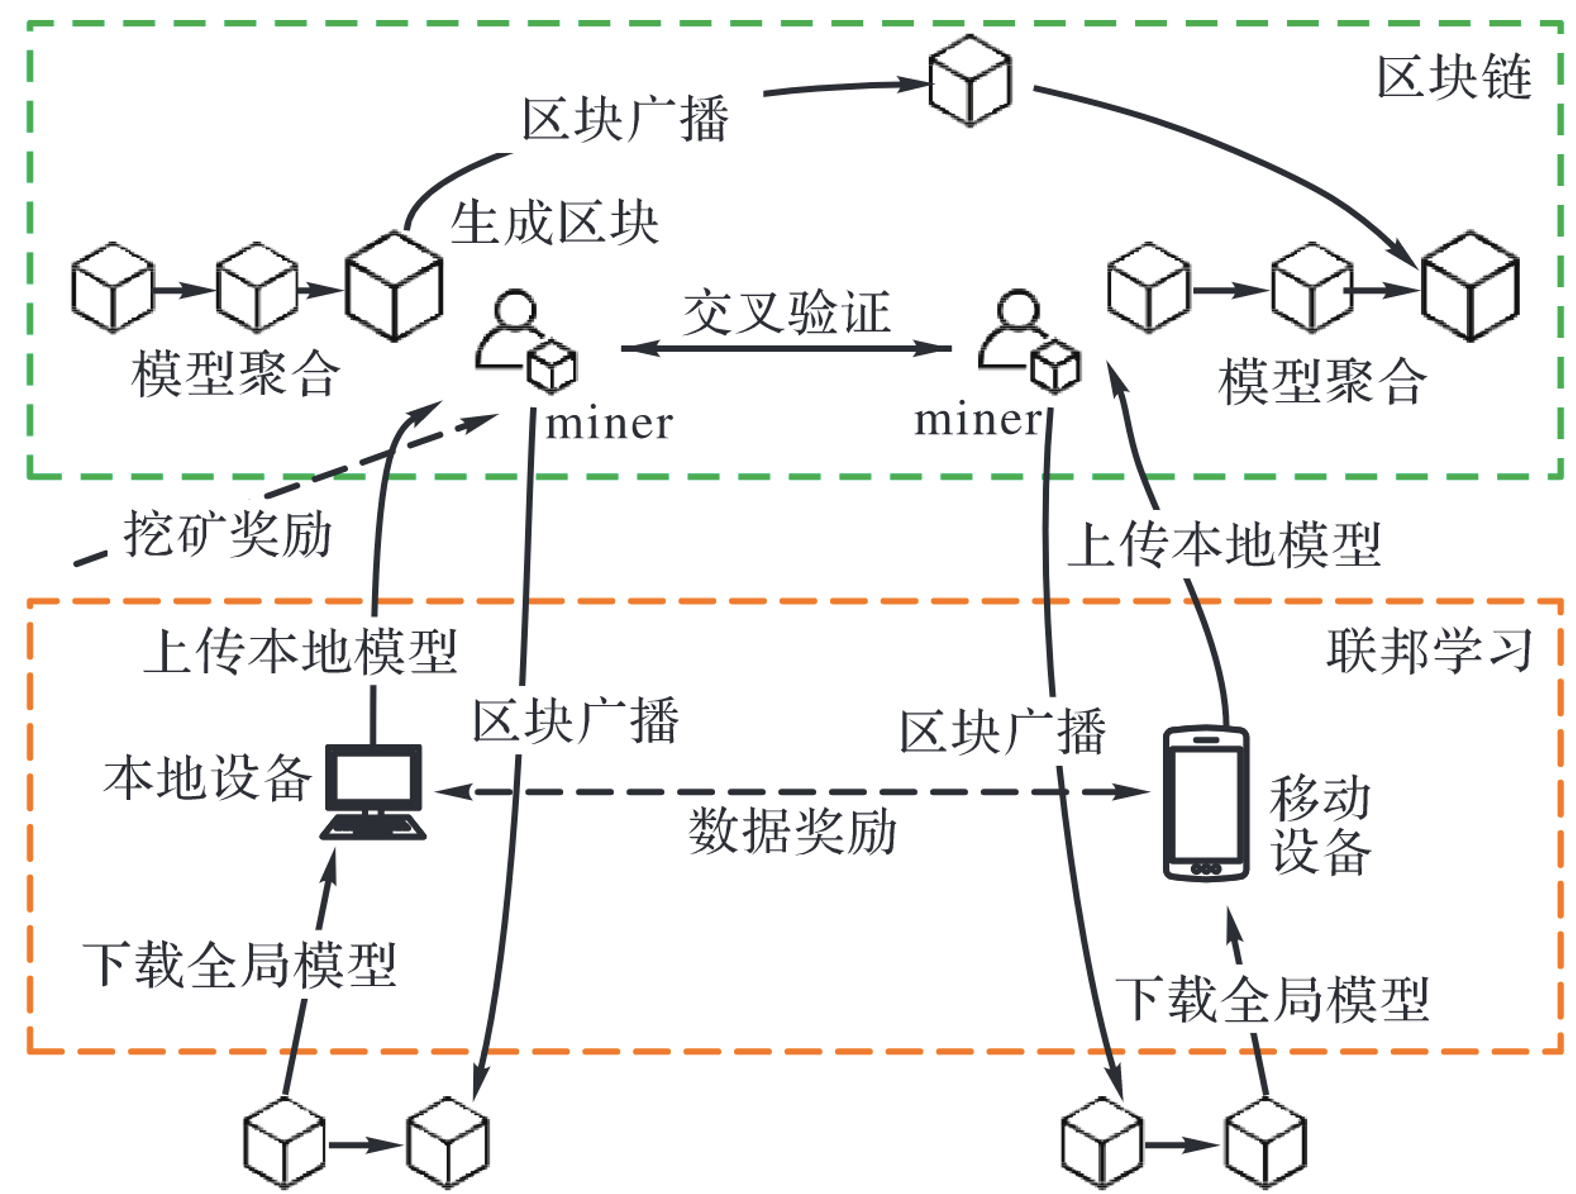
\includegraphics[width=1\textwidth]{images/blockchain}
\end{column}
\begin{column}{0.4\textwidth}
\textbf{利用区块链取代中央服务器}\\
用户将本地模型提交给维护区块链的矿工(Miner),矿工执行交叉验证、模型聚合等步骤,并基于共识机制生成一致的全局模型,随后利用区块存储和传播该全局模型,使用户能够从区块中将一致的全局模型下载到本地,进行下一轮训练。
\end{column}
\end{columns}
\end{frame}

\begin{frame}[fragile]{可行性分析}
\begin{itemize}
\item 研究方案的可行性
  \begin{itemize}
  \item 联邦学习可以很好的解决“数据孤岛”问题,适用于分布式轨迹数据的隐私保护。
  \item 采用差分隐私对用户的轨迹数据集进行加噪已经在领域内广泛运用。
  \item 采用区块链构建去中心化的联邦学习框架能够应对不可信环境下的隐私保护问题。
  \end{itemize}
\item 研究实验的可行性
  \begin{itemize}
  \item 拟采用GeoLife数据集与Porto数据集,度量指标采用JSD、MI、Top $N$ Visited Places、Accuracy、Precision、Recall、F1- Score。
  \item 拟使用联邦学习框架Flower: A Friendly Federated Learning Framework。
\end{itemize}
\begin{columns}
\begin{column}{0.7\textwidth}
\begin{block}{Code example from https://flower.dev/}<+->
\begin{lstlisting}[language=Python]
import flwr as fl
fl.client.start_numpy_client(server_address="[::]:8080", client=CifarClient())
fl.server.start_server(config=fl.server.ServerConfig(num_rounds=3))
\end{lstlisting}
\end{block}
\end{column}
\begin{column}{0.3\textwidth}

\includegraphics
[width=0.7\textwidth]{images/flower-logo}\\
\end{column}
\end{columns}
 
\end{itemize}

\end{frame}

\begin{frame}{研究基础}
本人所在单位福建工程学院拥有“福建省大数据挖掘与应用技术重点实验室” 等与本文直接相关的省级重点科研平台,同时本人受到了导师章静教授的\textbf{国家自然科学基金项目(619020690)}和\textbf{福建省自然科学基金项目(2021J011068)}的资金支持。目前的研究成果总结如下:
	\begin{itemize}
    	\item Zhang, J, Huang, Q, Huang, Y, Qian, D \& Tsai, P. (2022). DP-TrajGAN: A Privacy-Aware Trajectory Generation Model with Differential Privacy. Future Generation Computer Systems. (SCI 1区, 已录用) 
    	\item Zhang, J., Huang, Q., Hu, J. Y., \& Ye, X. C. (2022). Dimension-aware under spatiotemporal constraints: an efficient privacy-preserving framework with peak density clustering. The Journal of Supercomputing, 1-28. (SCI 3区, 已发表)
    	\item Xue, X., \& Huang, Q. (2022). Generative adversarial learning for optimizing ontology alignment. Expert Systems, e12936. (SCI 4区, 已发表)
   	\end{itemize}
   	
\end{frame}


\section{特色与创新}

\begin{frame}{本文的特色与创新之处}

\begin{itemize}
    \item 在大数据发布阶段,\textbf{基于差分隐私的轨迹生成模型}能够模拟出仿真轨迹从而替代真实轨迹进行发布,同时也能够保留原始轨迹的特征为下游各种类型的数据挖掘应用服务。
    \item 在分布式轨迹数据的场景下,\textbf{基于本地化差分隐私的联邦学习轨迹分类模型}能够解决“数据孤岛”问题,并且本地差分隐私技术能够使攻击者无法通过云端反推权重数据从而恢复本地数据。
    \item 在不可信的环境下,构建一种\textbf{基于区块链的可信联邦学习模型},使其能够有效利用区块链技术解决联邦学习的不可信及单点宕机问题,真正使得整体架构去中心化。
  \end{itemize}
\end{frame}



\backmatter

\end{document}
